\section{Практычны занятак №5}

\subsection{Структура праекта}

На малюнку \ref{img: pz5} прадстаўлена файлавая структура праекта.

\begin{figure}[h!]
    \centering
    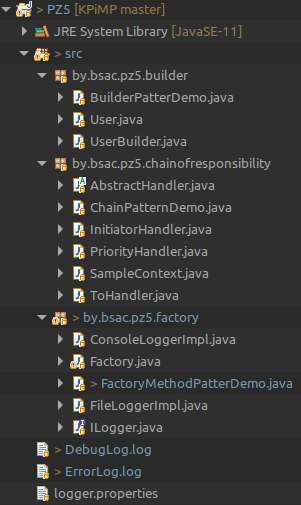
\includegraphics[width=0.5\textwidth]{pz5_structure}
    \caption{Файлавая структура практычнага занятку}
    \label{img: pz5} 
\end{figure}

\subsection{Заданне 1}

\subsubsection{Апісанне задання.}

Пры дапамозе шаблона \textit{Factory} рэалізаваць логіку,
якая выводзіць паведамленні ў \textit{debug} альбо ў \textit{error}
на экран альбо запісвае ў файл.

Інтэрфейс ILogger апісвае два асноўных метады debug з параметрам msg і error з параметрам msg, дзе msg - паведамленне, якое трэба вывесці на кансолі або запісаць у файл. Створаны два класы, такія як ConsoleLoggerImpl -- для вываду паведамлення на кансоль і FileLoggerImpl -- для запісу паведамлення ў файл. Так жа створаны клас Factory, які з дапамогай метаду getLogger вяртае FileLoggerImpl альбо ConsoleLoggerImpl на падставе ўласцівасці FileLogging = true (або false), што знаходзіцца у файле logger.properties. Калі значэнне true, то getLogger вяртае FileLoggerImpl, інакш ConsoleLoggerImpl. У класе FactoryMethodPatternDemo прыведзены прыклад выкарыстання шаблону Factory на практыцы.

У лістынгу \ref{lst: pz5_iLogger} прадстаўлены зыходны код інтэрфейса \textit{ILogger}.

\lstinputlisting[caption={Зыходны код інтэрфейса ILogger},%
                 label={lst: pz5_iLogger},%
                 language=java]{PZ5/Java/ILogger.java}

У лістынгу \ref{lst: pz5_consoleLoggerImpl} прадстаўлены зыходны код класа \textit{ConsoleLoggerImpl}.

\lstinputlisting[caption={Зыходны код класа ConsoleLoggerImpl},%
                 label={lst: pz5_consoleLoggerImpl},%
                 language=java]{PZ5/Java/ConsoleLoggerImpl.java}

У лістынгу \ref{lst: pz5_fileLoggerImpl} прадстаўлены зыходны код класа \textit{FileLoggerImpl}.

\lstinputlisting[caption={Зыходны код класа FileLoggerImpl},%
                 label={lst: pz5_fileLoggerImpl},%
                 language=java]{PZ5/Java/FileLoggerImpl.java}


У лістынгу \ref{lst: pz5_factory} прадстаўлены зыходны код класа \textit{Factory}.

\lstinputlisting[caption={Зыходны код класа Factory},%
                 label={lst: pz5_factory},%
                 language=java]{PZ5/Java/Factory.java}

У лістынгу \ref{lst: pz5_factoryMethodPatternDemo} прадстаўлены зыходны код класа \textit{Factory}.

\lstinputlisting[caption={Зыходны код класа FactoryMethodPatternDemo},%
                 label={lst: pz5_factoryMethodPatternDemo},%
                 language=java]{PZ5/Java/FactoryMethodPatternDemo.java}

\vspace{-\baselineskip}
\subsection{Заданне 2}

Пры дапамозе шаблона Builder стварыць клас, які можа ствараць
карыстальнікаў з уласцівасцямі, у залежнасці ад выкліканага канструктара.

У лістынгу \ref{lst: pz5_user} прадстаўлены зыходны код класа \textit{User}.

\lstinputlisting[caption={Зыходны код класа User},%
                 label={lst: pz5_user},%
                 language=java]{PZ5/Java/User.java}

У лістынгу \ref{lst: pz5_userBuilder} прадстаўлены зыходны код класа \textit{UserBuilder}.

\lstinputlisting[caption={Зыходны код класа UserBuilder},%
                 label={lst: pz5_userBuilder},%
                 language=java]{PZ5/Java/UserBuilder.java}

У лістынгу \ref{lst: pz5_builderPatternDemo} прадстаўлены зыходны код класа \textit{BuilderPatternDemo}.

\lstinputlisting[caption={Зыходны код класа BuilderPatternDemo},%
                 label={lst: pz5_builderPatternDemo},%
                 language=java]{PZ5/Java/BuilderPatterDemo.java}

\subsection{Заданне 3}


У лістынгу \ref{lst: pz5_AbstractHandler} прадстаўлены зыходны код класа \textit{AbstractHandler}.

\lstinputlisting[caption={Зыходны код класа AbstractHandler},%
                 label={lst: pz5_AbstractHandler},%
                 language=java]{PZ5/Java/AbstractHandler.java}

У лістынгу \ref{lst: pz5_ChainPatternDemo} прадстаўлены зыходны код класа \textit{ChainPatternDemo}.

\lstinputlisting[caption={Зыходны код класа ChainPatternDemo},%
                 label={lst: pz5_ChainPatternDemo},%
                 language=java]{PZ5/Java/ChainPatternDemo.java}

У лістынгу \ref{lst: pz5_InitiatorHandler} прадстаўлены зыходны код класа \textit{InitiatorHandler}.

\lstinputlisting[caption={Зыходны код класа InitiatorHandler},%
                 label={lst: pz5_InitiatorHandler},%
                 language=java]{PZ5/Java/InitiatorHandler.java}

У лістынгу \ref{lst: pz5_PriorityHandler} прадстаўлены зыходны код класа \textit{PriorityHandler}.

\lstinputlisting[caption={Зыходны код класа PriorityHandler},%
                 label={lst: pz5_PriorityHandler},%
                 language=java]{PZ5/Java/PriorityHandler.java}

У лістынгу \ref{lst: pz5_SampleContext} прадстаўлены зыходны код класа \textit{SampleContext}.

\lstinputlisting[caption={Зыходны код класа SampleContext},%
                 label={lst: pz5_SampleContext},%
                 language=java]{PZ5/Java/SampleContext.java}

У лістынгу \ref{lst: pz5_ToHandler} прадстаўлены зыходны код класа \textit{ToHandler}.

\lstinputlisting[caption={Зыходны код класа ToHandler},%
                 label={lst: pz5_ToHandler},%
                 language=java]{PZ5/Java/ToHandler.java}
